\section {Methodology}

\subsection{Glushko's Questions on Information Organisation}

\subsubsection{What is the main purpose of the website?}
The above the surface website focus to provide an interactive platform for users to explore the archaeological finds from the excavation of Amsterdam’s North-South metro line.

\subsubsection{Who is it for?}
The website is for anyone interested in archaeology, history, and Amsterdam’s heritage. The website has collections of items from different time period so can act as a gateway for collectors of ancient antique artifacts.

\subsubsection{Why it is being organized?}
Users can use the website to learn about the archaeological finds from the excavation of Amsterdam’s North-South metro line, view images of the artifacts, and read about their historical significance.

\subsubsection{Where it is being organized?}
The website provides information about the project, a timeline of the excavation, and a gallery of images of the artifacts found during the excavation

\subsubsection{How it is being organized?}
The website is organized into four main sections: Home, Project, Timeline, and Gallery. Each section has sub-sections that provide more detailed information.

\subsection{Data Dictionary and Metadata}

The below the surface website provides users with a data dictionary as part of the available data downloads \cite{BelowAmsterdam}.  However, the information provided was not sufficient for the needs of the project.  For example, the location of the sites related to the project code provided for each object.  However, there was no description provided of which project code related to which site.  It was only through research on the website that we were able to determine which site related to which project code.  The meta data provided was left unchanged, as the enriched description in the data dictionary met the needs of the project.

\subsection{Ontology} 
Development of the ontology consisted of 4 steps: Define scope, Enumerate important entities, Build the class hierarchy, and Specify the relationships between entities.

Six questions were posed to define and limit the scope of the ontology.  These questions were based on the needs identified by the user personas.
\begin{itemize}
    \item Where the finds are from?
    \item When are the finds from?
    \item Where are the finds found?
    \item What materials are the finds made of?
    \item What functional use does the find have?
    \item What weight do the finds have?
\end{itemize}

The ontology was developed in WebProtégé \footnote{https://webprotege.stanford.edu}.  As the ontology was developed the scope questions were used to ensure that additional aspects and classes were not investigated. The metadata fields in the data dictionary were used as a starting point, specifically those referring to the physical characteristics of the objects.  The other key metadata fields was the 'vondstnummer' or find number.  This is a unique identifier for each of the objects in the database.  It is created with a project code suffix.  This project code also relates to the location where the object was found during excavations.  The class names were also selected based on existing schema defined on the web \footnote{https://schema.org/}.  Where a pre-defined schema was not available, for example with metadata headers in database, rdfs:label was used.     

Once the key classes were listed, a hierarchy was created.  For example, trench, level, feature, and selection were all hierarchically sorted under each respective project code, as they related to the differing levels of location accuracy within each site. Once the classes and hierarchies had been listed, relationships between each were defined.  This was also at the point that defined schemas were linked to metadata headings found in the database. And relationships between dutch metadata names in the database with their English descriptions were made. For example the triple "put, rdfs:sameAs, trench.  With the established hierarchy and relationships as a foundation, the ontology was created over a number of iterations. To test the ontology, the WebWOWL web tool was used \footnote{https://service.tib.eu/webvowl/}.

\subsection{Data Model}

The data model for the website is designed to manage the archaeological finds efficiently. The primary goals of this data model are:

\begin{itemize}
\item Normalize the data to minimize redundancy and maintain data integrity.
\item Provide a unified structure for different material categories.
\item Enable the storage of common attributes shared by all archaeological finds.
\end{itemize}

 \begin{figure*}[!]
    \centering
    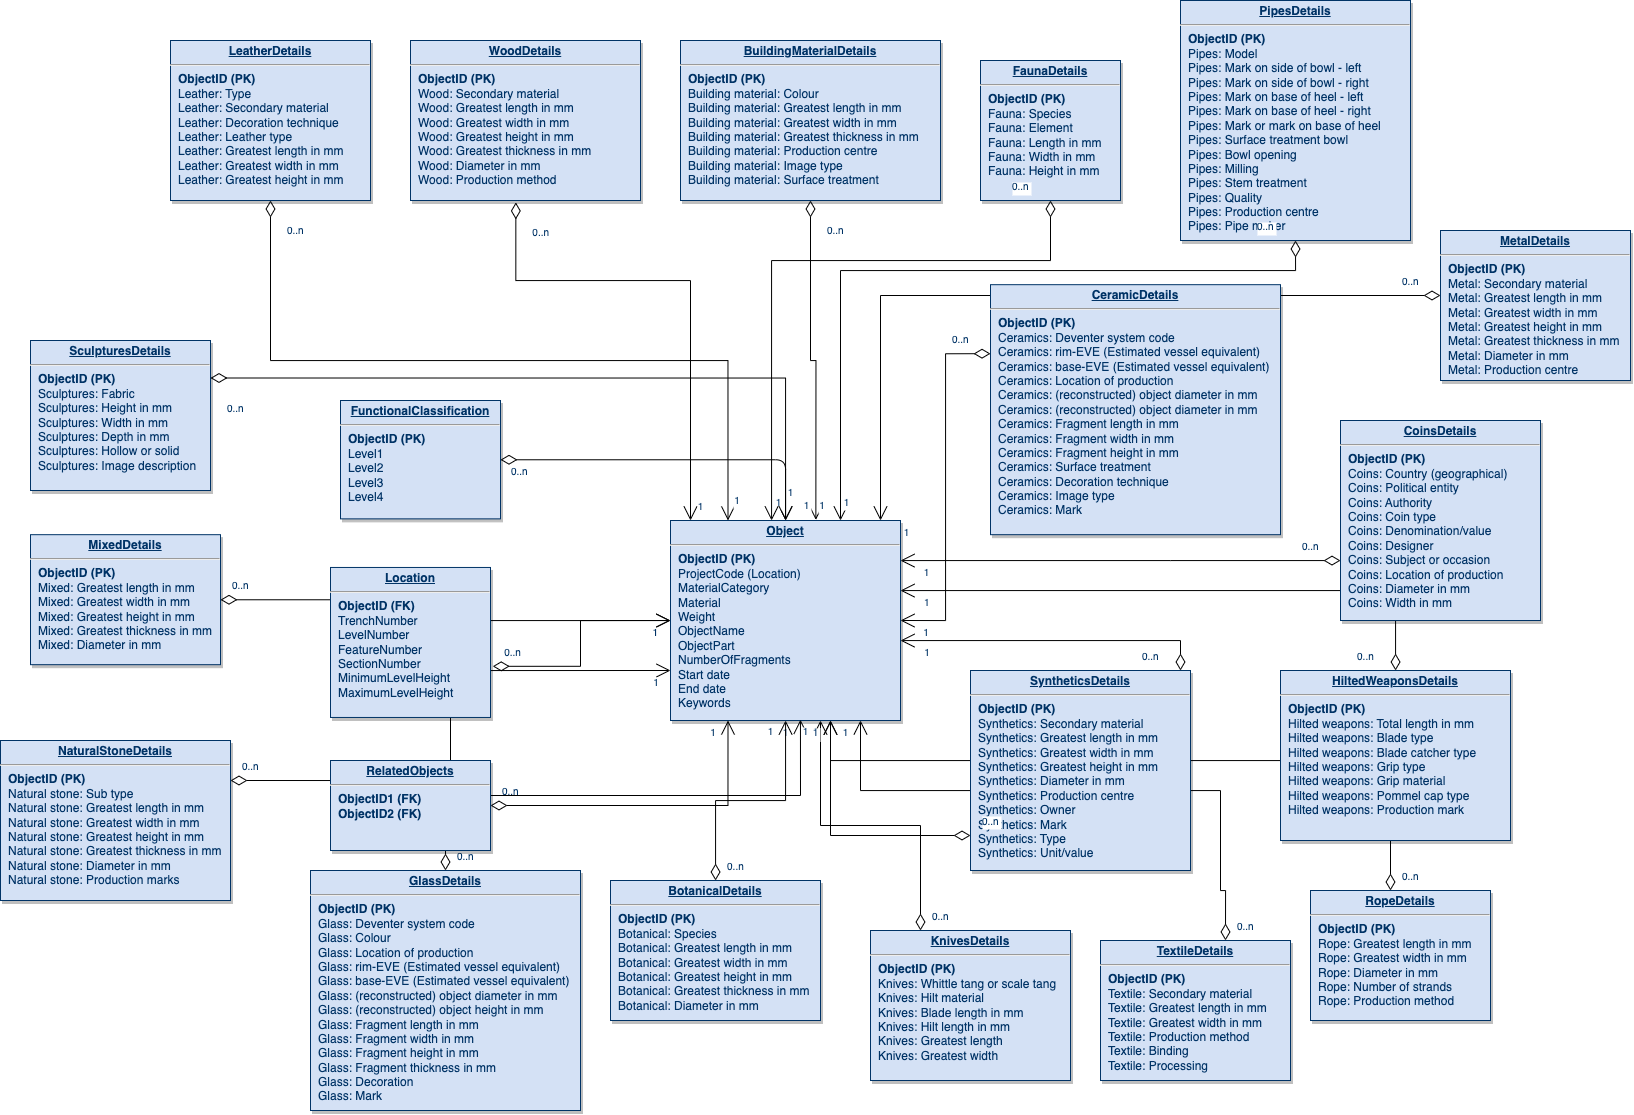
\includegraphics[width=0.8\paperwidth]{media/final data model.png}
    \caption{Data Model}
    \label{fig:data model}
\end{figure*}

The data model as shows in Figure \ref{fig:data model} is structured into following main parts:

\subsubsection{Object}
This table is central to the data organisation for common attributes of all archaeological finds. It includes information such as the ObjectID, project code, category, subcategory, weight, object name, object part, number of fragments, and temporal data (start date, end date). The ObjectID field acts as the identifier for all objects and is the primary key.

\subsubsection{Location}
This table contains fields for location information (trench number, level number, feature number, and section number), as well as keywords and classification levels. A binary field indicates whether the find is listed on the website. ObjectID is relating the location with Object as foreign key.

\subsubsection{Functional classification}
This table contains the main functional usage of the object. It is divided into catergories and level of functional classification between Level 1 to Level 4.

\subsubsection{Related Objects}
The "Related Objects" table is a critical component of the data model, as it enables the establishment of relationships between different archaeological finds. This table serves as a bridge to link findings that may have connections between each other. In the context of the model, it enables the website to visualize associations between artifacts and materials within and across categories.

\subsubsection{Material-Specific Tables}
Each material category (e.g., Ceramics, Glass, Building Materials, etc.) is represented by a dedicated table linked to the Object Table through a foreign key relationship. These material-specific tables store attributes that are unique to each category, including dimensions, production details, and any other specialized data relevant to the category.

\subsection{Technical Implementation of the website}

The website is a custom front-end mostly using web standards and open-source software and libraries. The assumption is that it will mainly be used in a desktop environment by the users to explore on larger screens so the website is not fully responsive and thus not mobile-optimized. 

\subsubsection{Front-end frameworks}
The web application is created with the open-source front-end framework Svelte \footnote{https://svelte.dev} and UI framework SvelteKit which allows the application to be built-in interface components, each chart is rendered separately making it more efficient to add functionality (e.g. add datasets, render different chart types) in the future but also makes the website performant when more data and charts are added. Svelte can be downloaded as a module (package) from NPM \footnote{https://www.npmjs.com} and uses the JavaScript back-end run-time Node.js \footnote{https://nodejs.org/}. For the charts the JavaScript charting library Chart.js \footnote{https://www.chartjs.org} is integrated into the components which allows charts to be rendered in HTML5 Canvas without much configuration. 

\subsubsection{Dataloading}
The processed and transformed dataset was used as a primary data source of which subsets of the dataset in \textit{.csv} format, roughly one per year chart and section, are converted to \textit{.json}. These data files are loaded on page load of the browser. For this prototype, no back-end was set up and no database queries are being made. Any filter options and updating of the charts are more custom, it uses JavaScript utility functions to allow the data to be pre-processed and have only the data change. 

\subsection{Machine Learning Model}
\subsubsection{Data-set presentation}
Bellow the surface provides a data-set\cite{BelowAmsterdam} of all the objects resulting from the excavations. The data is provided in the form of a .csv file, with 139190 rows and 163 columns. Each row corresponds to an object. Describing each object is well outside of the scope of the purposes of this section, however, an explanation of the relevant columns is necessary. \\
The following columns are relevant for the purposes of the ML model: 
\begin{itemize}
    \item vondstnummer - represents a unique inventory number, in the form of a string. Every object has a vondstnummer. Example: "NZC1.00001MTL001".
    \item  object -  a description of the contents of the object. Example: "sieve residue"
    \item  subcategorie - a categorisation of the object material. Example: "metal: copper alloy"
    \item objectdeel - describes the object type morphologically (if it is part of a bigger object, a set, etc). Example: "fragment"
    \item vlak\_min - Describes the minimum depth at which the object might have been found. Example: "-22.0"
    \item vlak\_max - Describes the maximum depth at which the object might have been found. Example: "-22.01"
    \item begin\_dat - The beginning of the interval of the estimated year of the object. Example: "1675.0"
    \item eind\_dat - End of the interval of the estimated year of the object. Example: "1725.0"
    \item niveau1 - The category in which the object is placed. Example:  "Communication \& Exchange"
\end{itemize}
For the columns \textit{object, subcategorie, objectdeel, vlak\_min, vlak\_max, begin\_dat, eind\_dat,  niveau1} there are rows in the dataset in which one or more of these columns are blank.  \\
The column \textit{niveau1} can take the value of one of 12 pre-determined categories, as well as the value "Not classified". As previously mentioned, there are rows where this column is blank. 
\subsubsection{Objectives}
Our objective is to create a machine-learning model that will complete the missing data for the "niveau1" column. This means that our model will predict a value in the niveau1 column, for the rows where currently that column is blank or has the value "Not classified". The prediction will be based on the values in the \textit{object, subcategorie, objectdeel, vlak\_min, vlak\_max, begin\_dat, eind\_dat,  niveau1} columns, which will act like input to the machine-learning model. 
\subsubsection{Deliverables}
In order to achieve our objectives, the following files are delivered: 
\begin{itemize}
    \item process\_dataset.py - a simple python script that takes the original 163 column .csv files and consolidates it into another .csv files that only contains the columns of interest. The name of this .csv file is "selected\_dataset.csv" 
    \item machine\_learning.py - this python script is the backbone of the machine-learning process. It is a more-complex script that does the following steps: 
        \begin{itemize}
            \item Loads the "selected\_dataset.csv" dataset
            \item Preprocess the data (completes the values with 0 or placeholders here they are blank", etc)
            \item Converts text stings to vectors
            \item Splits the data into unlabeled and labelled data based on the values in the "niveau1" column
            \item Splits the labelled data using a training, testing, and validation split
            \item Builds the ML model
            \item Compiles the model
            \item Trains the model
            \item Tests the model
            \item Predicts the values of niveau1 for the unlabelled data
            \item Saves the updated dataset into a file named predicted\_dataset.csv
        \end{itemize}
    \item predicted\_dataset.csv - a file containing the dataset in selected\_dataset.csv, but with the column selected\_dataset.csv fully completed. 
\end{itemize}
\subsubsection{Model description}
Given the problem, a relatively simple neural network model was chosen. It consists of 1 input layer, 2 hidden layers and one output layer. The input layer has 7 input neurons, coresponding to the following variables:
\begin{itemize}
    \item subcategorie
    \item object
    \item objectdeel
    \item vlak\_min
    \item vlak\_max
    \item begin\_dat
    \item eind\_dat
\end{itemize}
For the text fields, a Text-to-Vector conversion was necesarry. We used the word2vec\_model for that. The data of the other columns was normalised. \\
The hidden layers were composed of 10 neurons (dense layers) with a relu activation function. The outputted has 12 neurons, with a softmax activation function, each neuron corresponding to one of the 12 category values niveau1 can take. \\ 
The neural network was trained on the labelled data, using a 80 - 10 - 10 training - validation - testing split.
